%
% nichthauptideal2.tex
%
% (c) 2021 Prof Dr Andreas Müller, OST Ostschweizer Fachhochschule
%
\bgroup
\definecolor{darkgreen}{rgb}{0,0.6,0}
\begin{frame}[t]
\frametitle{Das Ideal $\langle 2,X\rangle \subset \mathbb{Z}[X]$}
\vspace{-12pt}
\begin{center}
\begin{tikzpicture}[>=latex,thick]

\def\c{\clip (-2.8,-2.0) rectangle (2.8,2.0);}

\def\labels{
	\fill[color=white,opacity=0.5] (1.5,-0.1) circle[radius=0.2];
	\node at (1.5,-0.1) {$1$};
	\fill[color=white,opacity=0.5] (-0.9,1.7) circle[radius=0.2];
	\node at (-0.9,1.7) {$X$};
	\fill[color=white,opacity=0.5] (0.8,0.7) circle[radius=0.2];
	\node at (0.8,0.7) {$X^2$};
}

\only<-3>{
\begin{scope}[xshift=3.0cm,yshift=1.9cm]
	\begin{scope}
	\c
	\node at (0,0)
	{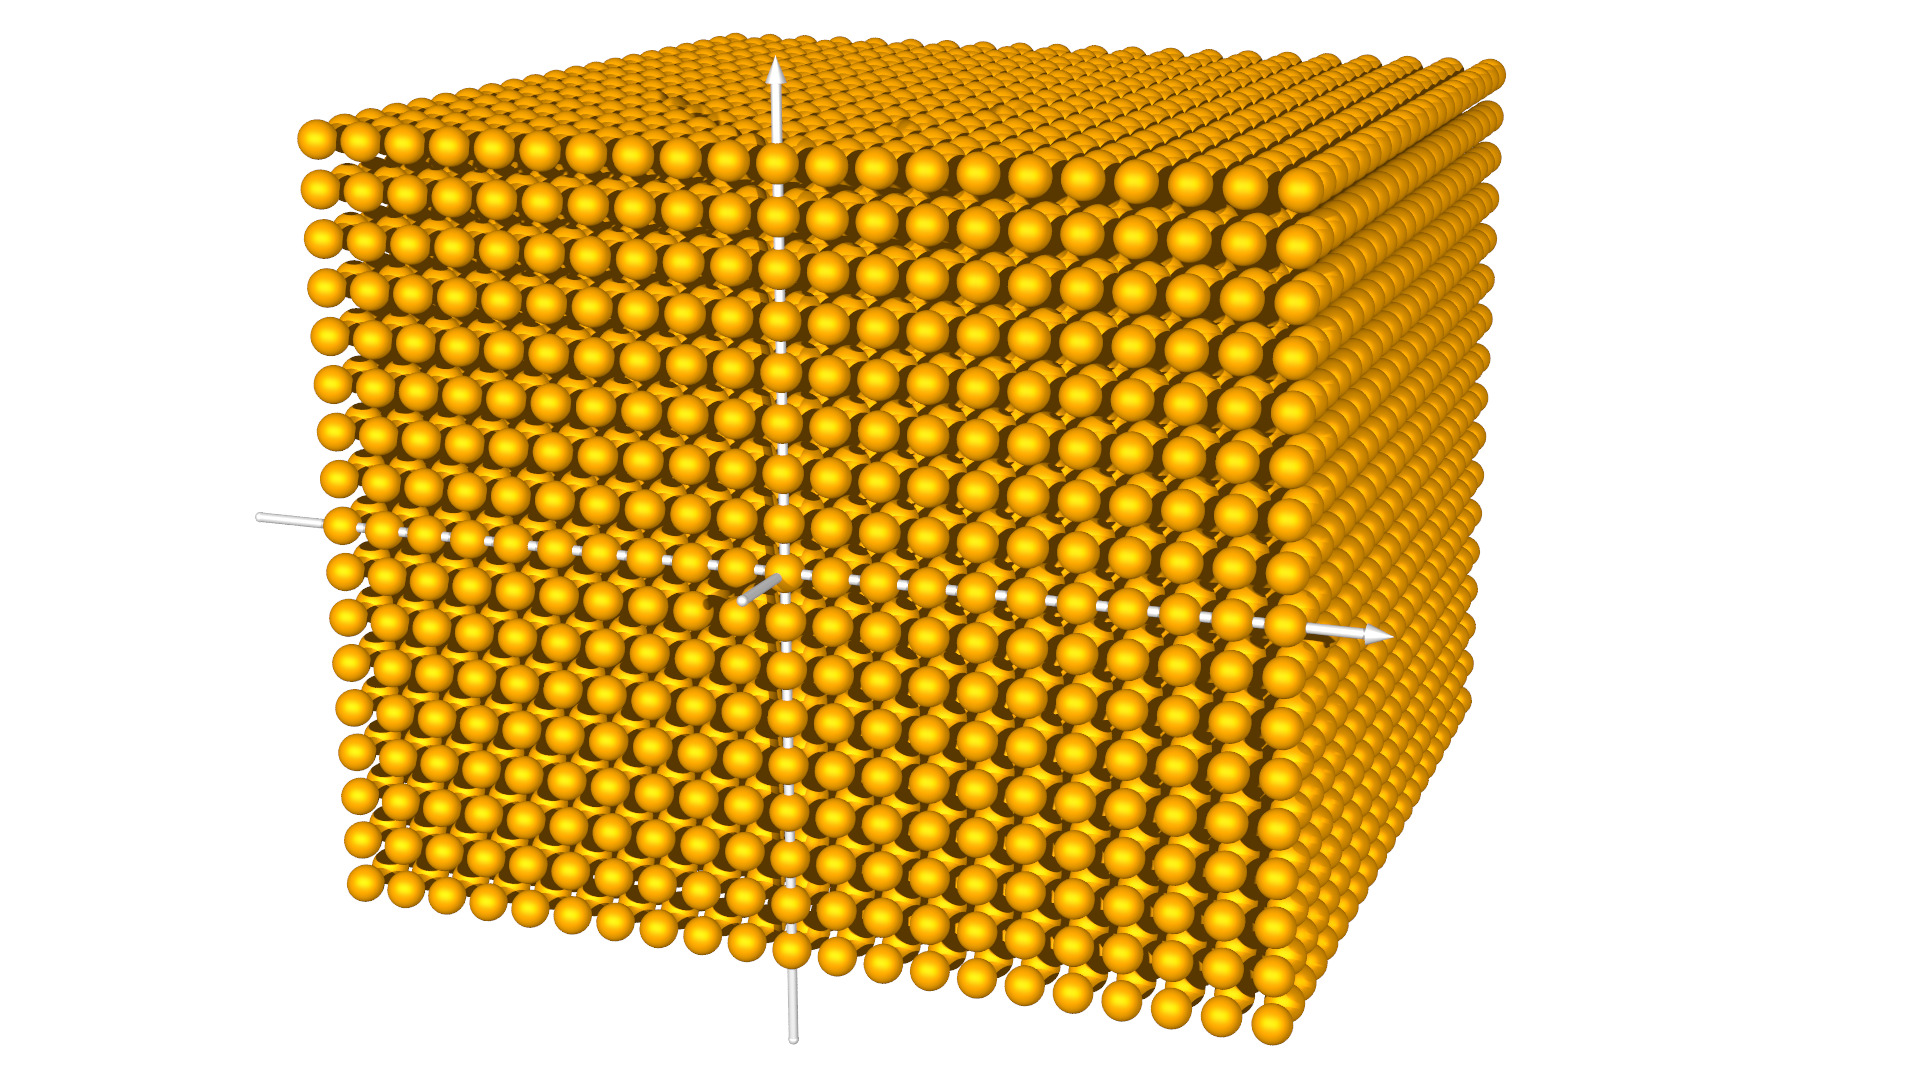
\includegraphics[width=7cm]{../slides/3/images/ring.jpg}};
	\end{scope}
	\node[color=orange] at (1.9,0.1) [right] {$\mathbb{Z}[X]$};
\end{scope}
}

\uncover<2->{
\begin{scope}[xshift=-3.0cm,yshift=1.9cm]
	\begin{scope}
	\c
	\node at (0,0)
	{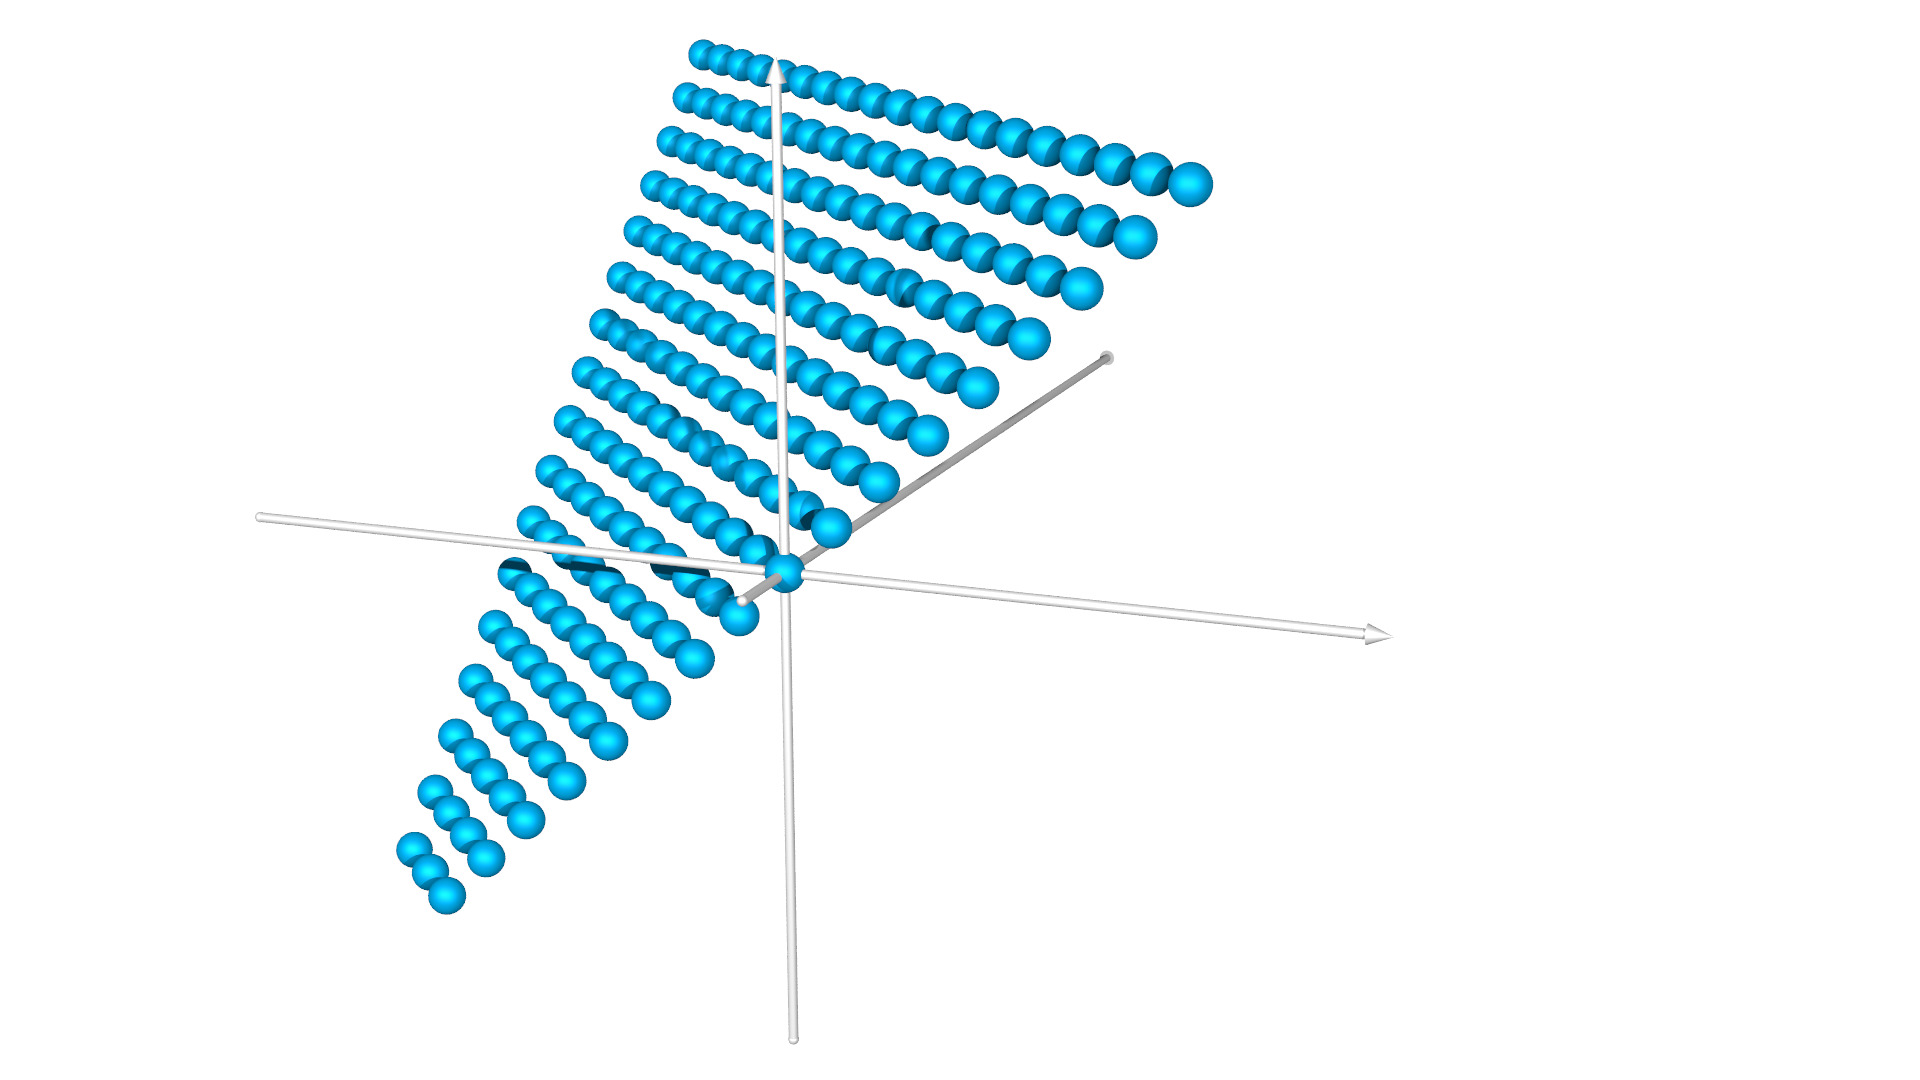
\includegraphics[width=7cm]{../slides/3/images/hauptideal.jpg}};
	\end{scope}
	\node[color=blue] at (-0.2,-1.2) {$(X+1)\cdot\mathbb{Z}[X]$};
	\labels
\end{scope}
}

\uncover<3->{
\begin{scope}[xshift=-3.0cm,yshift=-1.9cm]
	\begin{scope}
	\c
	\node at (0,0)
	{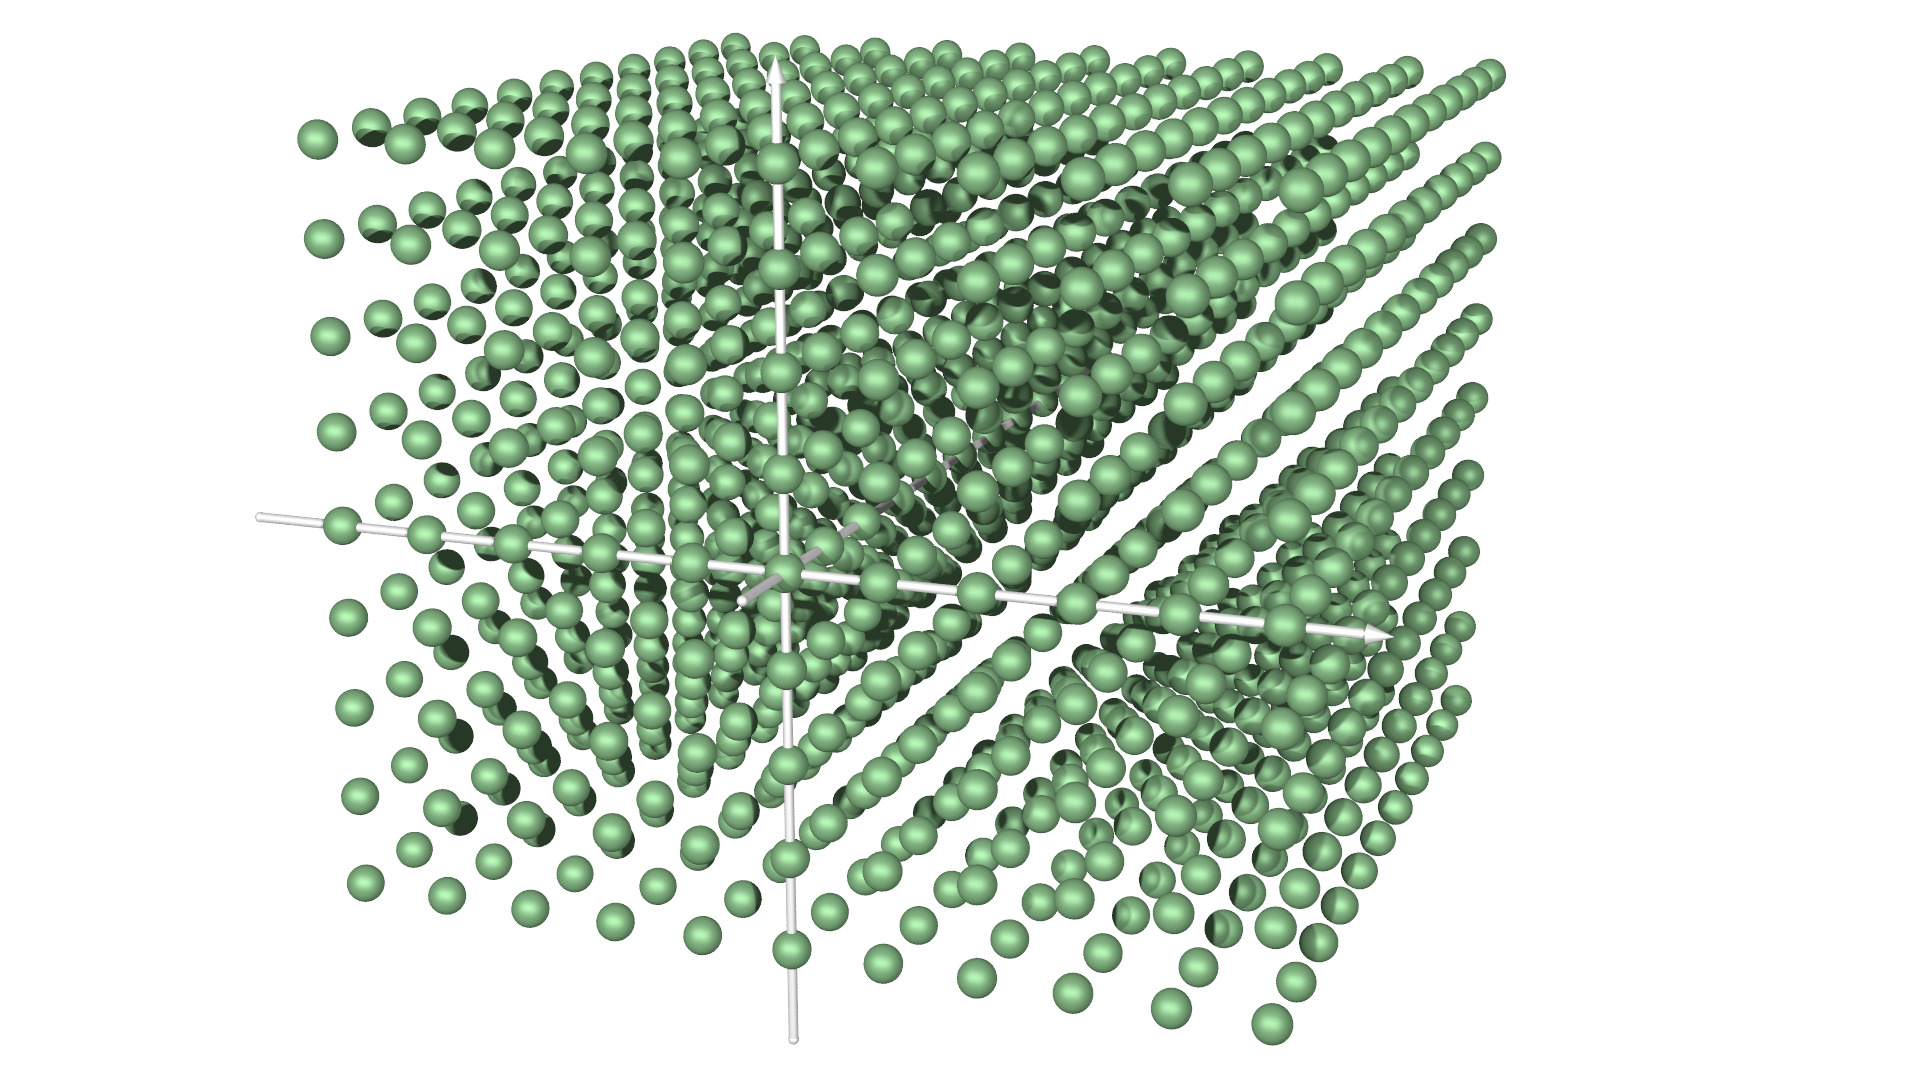
\includegraphics[width=7cm]{../slides/3/images/hauptideal2.jpg}};
	\end{scope}
	\node[color=darkgreen] at (-3.0,-0.8) {$2\cdot\mathbb{Z}[X]$};
\end{scope}

\begin{scope}[xshift=3.0cm,yshift=-1.9cm]
	\begin{scope}
	\c
	\node at (0,0)
	{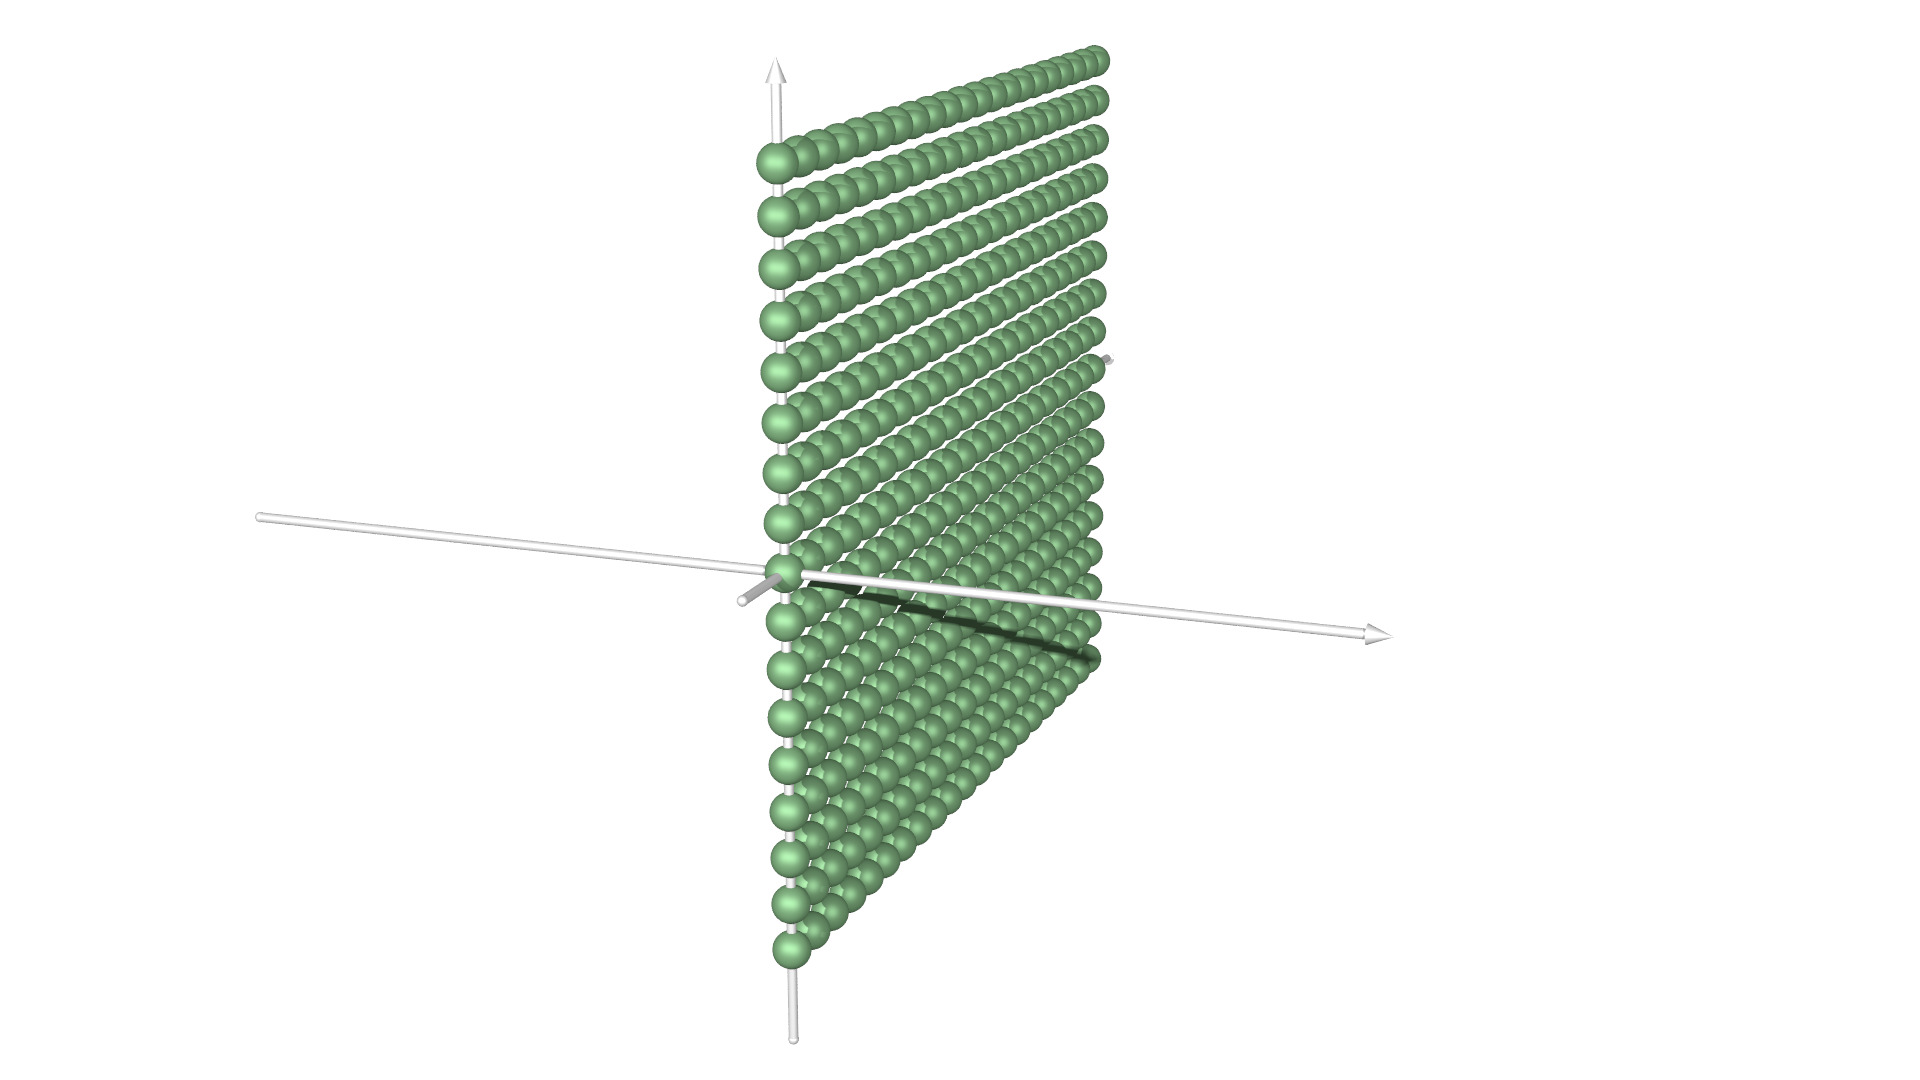
\includegraphics[width=7cm]{../slides/3/images/hauptidealX.jpg}};
	\end{scope}
	\node[color=darkgreen] at (2.5,-0.8) {$X\cdot\mathbb{Z}[X]$};
	\labels
\end{scope}
}

\uncover<4->{
\begin{scope}[xshift=3.0cm,yshift=1.9cm]
	\begin{scope}
	\c
	\node at (0,0)
	{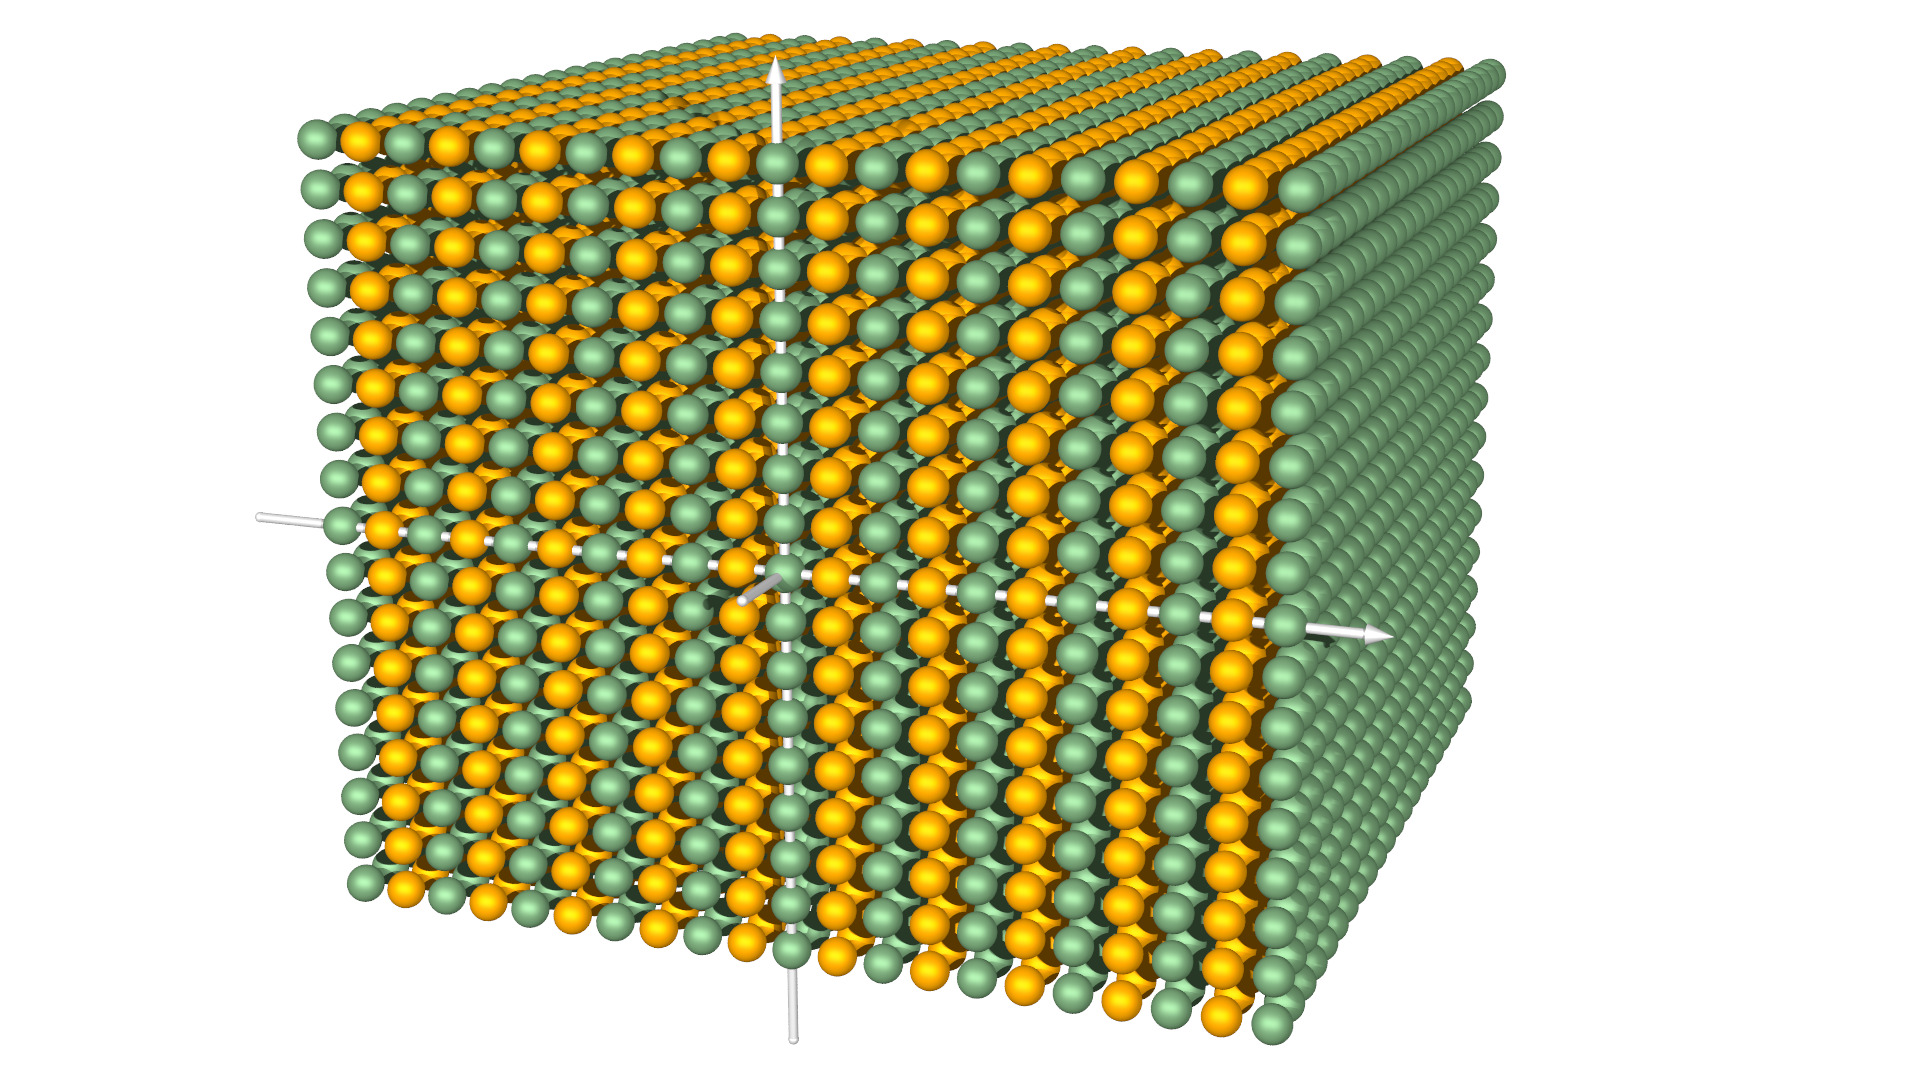
\includegraphics[width=7cm]{../slides/3/images/nichthauptideal.jpg}};
	\end{scope}
	\node[color=orange] at (1.9,0.1) [right] {$\mathbb{Z}[X]$};
	\node[color=darkgreen] at (1.9,-0.4) [right] {$\langle 2,X\rangle$};
\end{scope}
}

\draw[color=gray!50] (-6.6,0) -- (6.4,0);
\draw[color=gray!50] (0,-3.8) -- (0,3.8);

\begin{scope}[xshift=3.0cm,yshift=1.9cm]
	\fill[color=white,opacity=0.5] (1.5,-0.6) circle[radius=0.2];
	\node at (1.5,-0.6) {$1$};
	\fill[color=white,opacity=0.5] (-0.4,1.7) circle[radius=0.2];
	\node at (-0.4,1.7) {$X$};
\end{scope}

\end{tikzpicture}
\end{center}

\end{frame}
\egroup
